\documentclass[11pt]{cernrep}
%\documentclass[12pt,letterpaper,twoside]{article}
%\documentclass[12pt,letterpaper]{article}
%\usepackage[pdftex]{graphicx,color}
\usepackage[pdftex]{graphicx,epsfig}
%\usepackage[dvips]{graphicx,color}
%\input{psfig}
%\input{epsf}
\usepackage{amsmath,amssymb}
%\usepackage[twoside,pdftex,letterpaper,text={6.5in,9in}]{geometry}
%\usepackage[twoside,dvips,letterpaper,text={6.5in,9in}]{geometry}
\usepackage[dvips,letterpaper,text={6.5in,9in}]{geometry}
\usepackage{fancyhdr}
\usepackage{verbatim}
\renewcommand{\baselinestretch}{1.1}
%\renewcommand{\theequation}{\thesection.\arabic{equation}}
%\numberwithin{equation}{section}

%       Symbol definitions
\newcommand\ltap{\
  \raise.3ex\hbox{$<$\kern-.75em\lower1ex\hbox{$\sim$}}\ }
\newcommand\gtap{\
  \raise.3ex\hbox{$>$\kern-.75em\lower1ex\hbox{$\sim$}}\ }
 \newcommand{\sss}{\scriptscriptstyle}
 \renewcommand{\phi}{\varphi}
%%%%%%%%%%%%%%%%%%%%%%%%%%%%%%%%%%%%%%%%%%%%%%%%%%%%%%%%%%%%%%%%%%%%%%%%

%  \simge and \simle make "approx greater than" and "approx less than"
\newcommand\simge{\mathrel{%
   \rlap{\raise 0.511ex \hbox{$>$}}{\lower 0.511ex \hbox{$\sim$}}}}
\newcommand\simle{\mathrel{
   \rlap{\raise 0.511ex \hbox{$<$}}{\lower 0.511ex \hbox{$\sim$}}}}

%  \slashcar puts a slash through a character to represent contraction
%  with Dirac matrices. Use \not instead for negation of relations, and use
%  \hbar for hbar.
\newcommand{\slashchar}[1]%
        {\kern .25em\raise.18ex\hbox{$/$}\kern-.75em #1}
%%%%%%%%%%%%%%%%%%%%%%%%%%%%%%%%%%%%%%%%%%%%%%%%%%%%%%%%%%%%%%%%%%%%%%%%%%
\def\lsim{\mathrel{\raise.3ex\hbox{$<$\kern-.75em\lower1ex\hbox{$\sim$}}}}
\def\gsim{\mathrel{\raise.3ex\hbox{$>$\kern-.75em\lower1ex\hbox{$\sim$}}}}
%%%%%%%%%%%%%%%%%%%%%%%%%%%%%%%%%%%%%%%%%%%%%%%%%%%%%%%%%%%%%%%%%%%%%%%%%%
\newcommand{\bs}{\boldsymbol}

\newenvironment{changemargin}[2]{\begin{list}{}{
        \setlength{\topsep}{0pt}\setlength{\leftmargin}{0pt}
        \setlength{\rightmargin}{0pt}
        \setlength{\listparindent}{\parindent}
        \setlength{\itemindent}{\parindent}
        \setlength{\parsep}{0pt plus 1pt}
        \addtolength{\leftmargin}{#1}\addtolength{\rightmargin}{#2}
        }\item }{\end{list}}
%
\begin{document}
\title{
%\vskip -15mm
Simplified Template Cross Sections: sensitivity to dimension-6 interactions at LHC run 2}
\author{Jorge~de~Blas$^{1,2}$,
Kristin~Lohwasser$^3$, Pasquale~Musella$^4$ and Ken~Mimasu$^5$}
\institute{$^1$Dipartimento di Fisica e Astronomia ``Galileo Galilei'', Universit\`a di Padova,\\ Via Marzolo 8, I-35131 Padova, Italy\\
$^2$INFN, Sezione di Padova, Via Marzolo 8, I-35131 Padova, Italy\\
$^3$Department of Physics and Astronomy, Sheffield University, Sheffield, UK \\
$^4$Institute for Particle Physics and Astrophysics, ETH Zurich, CH\\
$^5$Centre for Cosmology, Particle Physics and Phenomenology (CP3), Universit\'e
catholique de Louvain, Chemin du Cyclotron, 2, B-1348 Louvain-la-Neuve, Belgium } 
\maketitle

\begin{abstract}
We perform a sensitivity study of the simplified template cross section (STXS) measurements to dimension-6 interactions within the standard model effective field theory framework. We focus on energy dependent effects in Higgs production in association with a $Z$-boson, $p p \to Z h \to \ell^+\ell^- b\bar{b}$. Several benchmark points are considered, with different values of a representative Wilson coefficient, alongside the Standard Model prediction as well as the dominant $Z+b\bar{b}$ background. We contrast the expected sensitivity obtained by the STXS to an optimised analysis exploiting multivariate techniques via a boosted decision tree classifier. The aim of this exercise is to estimate the amount information retained in the STXS binning, an therefore the power of the framework for model-independent hypothesis testing in Higgs physics. \textbf{what did we find?}
\end{abstract}

%%%%%%%%%%%%%%%%%%%%%%%%%%%%%%%%%
%%%%%%%%%%%%%%%%%%%%%%%%%%%%%%%%%

\newpage

\section{Introduction}
\label{sec:intro}
% All
The Standard Model Effective Field Theory (SMEFT) is, by now, a well established framework for parametrising new physics effects in the interactions of Standard Model (SM) particles in a model independent way. It has been and continues to be a key part of the LHC programme, complementary to direct searches for new physics. The framework employs an operator expansion in canonical dimension suppressed by a generic cutoff scale, $\Lambda$, assumed to be much larger than the electroweak (EW) scale, situated by the vacuum expectation value of the Higgs field, $v$. The SM Lagrangian is thus supplemented by higher dimension operators and truncated at dimension-6, the lowest dimension at which $B$- and $L$-number conserving operators appear.
\begin{align}
    \mathcal{L}=\mathcal{L}_{SM}+\sum_i \frac{c_i}{\Lambda^2}\mathcal{O}^i_{D=6}+\cdots,
\end{align} 
Where the dimension-5 Weinberg operator for neutrino masses has been neglected. New physics effects are then expected to appear scaling between $\sim v^2/\Lambda^2$ and a heightened energy dependence of $\sim E^2/\Lambda^2$.

One of the main strengths of the LHC in this respect is its ability to probe the high energy regime, in which it is expected that the sensitivity to EFT effects will be maximised to the large momentum flow through the modified  vertices accessing the stronger energy growth of the higher dimensional operators. Furthermore, the discovery of the Higgs boson in 2012 has opened a brand new avenue in constraining the SMEFT parameter space consisting of the various operators involving Higgs fields. Measurements of Higgs production and decay modes have already provided new constraints on many operators and have also helped to constrain some blind directions in existing fits to low-energy data such as precision electroweak measurements at LEP. 

In the first run of the LHC, a very successful programme of signal strength measurements took place, in which information from many searches was combined into a global fit to overall coupling modifiers between the Higgs and the rest of the SM particles. The natural evolution of these measurements for Run 2 is to subdivide the phase space and work towards differential observables in Higgs production and decay. To this end, a staged approach termed Simplified Template Cross Sections (STXS) is being developed~\cite{deFlorian:2016spz}, consisting of an increasingly fine-grained binning of kinematic observables, separated by production and decay mode. The aim is to provide measurements in mutually exclusive regions of phase space, performed in simplified fiducial volumes and unfolded to remove detector and acceptance effects. Ideally, these will be designed to maximise sensitivity to new physics.

Being one of the main elements of LHC searches for non-SM physics, it is of great interest to evaluate the sensitivity of the STXS measurements to SMEFT effects in Higgs boson interactions, particularly since they will be able to access these high energy tails of kinematic distributions. In particular, one would like to know how the information provided by a generic framework such as the STXS would compare to an optimised, dedicated search for SMEFT effects. Naively, one may expect some loss of information given, \emph{e.g.}, the finite binning of the distributions. In this study, we aim to quantify this difference by comparing and contrasting the ability to constrain SMEFT effects in Higgs production between the STXS measurements and an optimised analysis making use of multivariate methods to extract the maximum classification power of the SMEFT signals. We consider the concrete scenario of the (ZH) production of a Higgs boson decaying into a pair of $b$-quarks in association with a $Z$-boson  decaying to a pair of leptons, in the presence of a single EFT operator. We simulate several benchmark values for the operator Wilson coefficient within existing constraints from global fits along with the dominant reducible SM background and evaluate the statistical discriminating power of a hypothesis test using the STXS measurements versus a multivariate Boosted Decision Tree (BDT) classifier.

The paper is organised as follows. We first describe the Monte Carlo event generation procedure for the SM and EFT benchmarks in section~\ref{sec:gen}. Section~\ref{sec:tools} first describes the fiducial selection employed, the training and analysis implemented using the BDT classifier and the STXS binning used for ZH. In Section~\ref{sec:test}, we summarise the results of the selections and binning and perform a statistical hypothesis test to quantify the relative strengths of the two methods before concluding and laying out the avenues for further investigation in Section~\ref{sec:conclusions}

\section{Generated Models} 
\label{sec:gen}
%Ken
%!TEX root = /Users/Ken/Work/Projects/LesHouches2017/STXSvsEFT/repo/LHStxsVsEft/Documentation/STXSvsSpecificEFTAna.tex
The production of a Higgs boson in association with an EW gauge boson can be considered one of the canonical LHC processes sensitive to SMEFT effects. Evidence for this process involving the $b\bar{b}$ decay mode of the Higgs and leptonic vector boson decays was finally observed in 2017~\cite{Aaboud:2017xsd,Sirunyan:2017elk}. Some of the operators which modify the Higgs coupling to these gauge bosons introduce $E^2/\Lambda^2$ effects in the production rate, enhancing it at high energies.
The associated production process can naturally access this region of phase space since the Higgs is produced recoiling against the associated vector, meaning that the $p_T$ of the Higgs or vector boson are a faithful proxy for the energy flowing through the EFT vertex. Of the many dimension-6 operators that can contribute to this process, we consider 
\begin{align}
    \mathcal{O}_{\sss HW} &= 
    \frac{ig}{2\Lambda^2} \big[D_\mu \phi^\dag \sigma_{k} D_\nu \phi\big] 
    W^{k,\mu \nu},
\end{align}
an operator from the so called strongly interacting light Higgs (SILH) basis~\cite{Giudice:2007fh,Contino:2013kra}. Here, $\sigma_{k}$ refers to the Pauli matrices and the covariant derivative, $D_\mu$, for the Higgs field is defined as
\begin{align}
    D_\mu\phi &= \partial_\mu \phi -  i g \frac{\sigma_{k}}{2} W_\mu^k \phi - \frac12 i g' B_\mu \phi,
\end{align}
with $g$ and $g^\prime$ the weak and hypercharge gauge couplings respectively.

A global fit~\cite{Ellis:2014jta} combining information from precision measurements at LEP and LHC Run 1 data constrains the Wilson coefficient, $c_{\sss HW}$, to lie in the range 
\begin{align}
    \frac{m_{\sss W}^2}{\Lambda^2}c_{\sss HW} = [-0.07,\,0.03].
\end{align}
A sensitivity estimate for LHC Run 2 was also performed in~\cite{Degrande:2016dqg} by projecting an 8 TeV ZH analysis~\cite{TheATLAScollaboration:2013lia} to 13 TeV. The results of the study indicated that the previous bound could be improved by an order of magnitude. This indicates that the STXS measurements are likely to provide even greater sensitivity to this parameter.

Motivated by the limits from the global fit, we select the following benchmark values for $c_{\sss HW}$:
\begin{align}
    C_{\sss HW} = \pm 0.03 \text{ and } \pm0.01\,,
\end{align}
with $ C_{\sss HW}\equiv c_{\sss HW} m_{\sss W}^2/\Lambda^2$. The first value roughly saturates the positive end of the limit, and has been shown to yield drastic effects in the kinematic tails of distributions~\cite{Degrande:2016dqg}. The second corresponds to a smaller, yet potentially accessible value of the parameter that may better test the relative discriminating power of relatively small effects between the two methods we investigate. We simulate our Monte Carlo samples at leading order using {\sc MadGraph5\_aMC@NLO}~\cite{Alwall:2014hca} with the public {\sc HELatNLO}~\cite{Degrande:2016dqg,Alloul:2013naa} {\sc FeynRules}~\cite{Alloul:2013bka} model, exploiting reweighting methods to simulate multiple parameter space points (including the SM) simultaneously. We also include the dominant irreducible background contribution from $Z b\bar{b}$ production with the $Z$-boson decaying leptonically. Showering and hadronisation, as well as the Higgs boson decay to $b\bar{b}$ are performed with {\sc PYTHIA8}~\cite{pythia8} and the events are reconstructed from hadron level with {\sc MadAnalysis5}~\cite{Conte:2012fm} which makes use of {\sc FastJet}~\cite{Cacciari:2011ma}.



\section{Analysis}
\label{sec:tools}
\begin{itemize}
    \item Fiducial selection \& smearing
    \item subsection: BDT training methods \& classifiers
    \item subsection: STXS binning post Zbb classifier
\end{itemize}
%!TEX root = /Users/Ken/Work/Projects/LesHouches2017/STXSvsEFT/repo/LHStxsVsEft/Documentation/STXSvsSpecificEFTAna.tex
To begin the analysis on a realistic level, we first perform a simple fiducial selection on the event samples, to emulate a typical LHC selection that would be performed for the ZH process. To this end, we also implement a $p_T$ and $|\eta|$ dependent smearing function on the $b$-jet momenta to approximate finite detector resolution effects following the parametrised functions determined by the CMS particle-flow performance analysis~\cite{Sirunyan:2017ulk}.

Jets are clustered with the anti-$k_T$ algorithm with a radius parameter of 0.4 and required to have $p_T > 20$ GeV. Events are required to have two leptons satisfying $p_T > 25$ GeV and $|\eta|< 2.5$. Exactly two $b$-jets, as identified using truth-level information by {\sc MadAnalysis5}, are required satisfying $p_T > 20$ GeV and $|\eta|< 2.5$. We assume a flat $b$-tagging efficiency of $70\%$, corresponding to the DeepCSV medium working point defined in~\cite{Sirunyan:2017ezt}. Additionally, $Z$- and Higgs-boson mass windows are imposed on the invariant masses of the lepton and $b$-jet pairs such that $75 < M_{\ell\ell} < 105$ GeV and  $60 < M_{\ell\ell} < 140$ GeV. This defines our fiducial volume on which both the BDT training and STXS binning will be performed. Table~\ref{tab:FiducialXS} summarises the cross sections obtained after the fiducial selection for the Monte Carlo samples generated. The $H\to b\bar{b}$ branching fraction is computed in the SM and the SMEFT benchmark points using the e{\sc HDECAY}~\cite{Contino:2014aaa} interface of {\sc Rosetta}~\cite{Falkowski:2015wza} and folded into the cross section results.
%
\begin{table}[h!]
    \centering
    \begin{tabular}{|l|l|}
        \hline
        $pp\to b\,\bar{b}\,\ell^+\,\ell^-$& $\sigma_{\text{fid.}} [fb]$\tabularnewline
        \hline
        $ZH$ SM&2.72\tabularnewline
        $ZH$ $c_{\sss HW} = 0.03$&3.64\tabularnewline
        $ZH$ $c_{\sss HW} = -0.03$&2.21\tabularnewline
        $ZH$ $c_{\sss HW} = 0.01$&3.38\tabularnewline
        $ZH$ $c_{\sss HW} = -0.01$&2.50\tabularnewline
        $Z b\bar{b}$ SM&291.3\tabularnewline
        \hline
    \end{tabular}
    \caption{\label{tab:FiducialXS} Cross sections obtained at LO after imposing the fiducial selection cuts described in Section\ref{sec:tools}.}
\end{table}
Clearly, the $Z b\bar{b}$ background is overwhelmingly large even after the Higgs mass
window selection. A realistic analysis will employ multivariate analyses techniques to
reduce this background. As explained in the next section, we mimic this aspect of the
experimental analyses by training a BDT discriminant to optimally reject this background
in favour of the SM $ZH$ process.


\clearpage
%!TEX root = /Users/Ken/Work/Projects/LesHouches2017/STXSvsEFT/repo/LHStxsVsEft/Documentation/STXSvsSpecificEFTAna.tex
We build a set of gradient BDT classifiers to efficiently discriminate
between the different event hypotheses involved in the analysis, namely $Z b\bar{b}$,
SM $Z H$, and BSM $Z H$ production. 
The classifiers receive kinematic variables related to the event as inputs and approximate
the likelihood for each event to belong to any of the three classes.

\begin{equation}
p_{i}(\vec x) = \frac{ e^{\beta_{i}(\vec x) } }{ \sum_j e^{\beta_{j}(\vec x) } }
\end{equation}
here $\vec x$ represents all the input variables to the discriminant, that are shown in
Table~\ref{tab:bdt_features} and $\beta_{i}(\vec x)$ are non-linear functions of these
variables.

These kind of algorithms are regularly used by the experimental analyses and often provide a comparable performance to those of more sophisticated techniques such as matrix element methods. 
%
\begin{table}[h!]
\centering
\begin{tabular}{||c|c||c|c||}
variable definition & variable name &  variable name & variable definition \\
\hline
$p_T(l_1)$ & leading lepton $p_T$ & $p_T(l_2)$ & sub-leading lepton $p_T$\\
$p_T(b_1)$ & leading b-jet $p_T$ & $p_T(b_2)$ & sub-leading b-jet $p_T$\\
$\eta(l_1)$ & leading lepton pseudo-rapidity & $\eta(l_2)$ & sub-leading lepton pseudo-rapidity\\
$\eta(b_1)$ & leading b-jet pseudo-rapidity  & $\eta(b_2)$ & sub-leading b-jet  pseudo-rapidity\\
$y(Z)$ & Z-candidate rapidity  & $y(H)$ & H-candidate rapidity \\
$p_T(Z)$ & Z-candidate $p_T$  & $m_{bb}$ & H-candidate invariant mass \\
$m_{VH}$ & HZ invariant mass  &  &  \\
\end{tabular}
\caption{
\label{tab:bdt_features}
Input variables used by the kinematic BDT discriminants.
}
\end{table}

Five sets of discriminants were trained:
\begin{enumerate}
\item A binary discriminant to separate $Z b\bar{b}$ production from the SM $Z H$ production.
\item Four sets of three-class discriminants (one for each of the $c_{\sss HW}$ benchmarks) to
    discriminate between $Z b\bar{b}$, SM $Z H$ and BSM $Z H$ production.
\end{enumerate}
The first discriminant was used to reduce the $Z b\bar{b}$ background in the template
cross section analysis, in such a way to mimic the experimental analyses.
The last four discriminants were used to first reduce the $Z b\bar{b}$ background and then to further classify the selected events to discriminate between the SM and BSM hypotheses.

The BDTs were trained using the scikit-learn~\cite{scikit-learn} and xgboost packages~\cite{xgboost}. To this end, the events were
split into two statistically independent samples, with a ratio of 3:1, used respectively for training and
application of the discriminants. % Three quarters of the events were used for training.
We used the categorical cross-entropy loss function, and the algorithm hyperparameters were
optimised on the training sample using stochastic grid search and the mean
k-fold cross-validation loss as figure of merit, with $k = 5$.
The optimized hyperparameters are shown in Table~\ref{tab:bdt_hpars}.

\begin{table}
\centering
\begin{tabular}{||c|c||}
parameter & value \\
\hline
number of trees & 600 \\
maximum depth & 5 \\
bagging fraction & 0.8 \\
learning rate & 0.05 \\
$L_2$ regularisation strength & 1 \\
\end{tabular}
\caption{
\label{tab:bdt_hpars}
Optimized BDT training hyperparameters.
}
\end{table}

After training, the $p(Z b\bar{b})$ variables were used to define selection criteria
for the events to be considered for analysis. The maximum allowed value for $p(Z b\bar{b})$
was determined in order to maximise the quantity $\varepsilon^2(SM Z H) / \varepsilon(Z
b\bar{b})$, where $\varepsilon$ is the selection efficiency of a given sample. Such a
figure of merit is, in the gaussian limit, proportional to the squared median expected
discovery significance to observe the standard model production of of $Z H$.
The choice was made again to mimic the experimental analyses, for which the observation of
the SM Higgs signal will be the primary goal.

In order to ensure a smooth behaviour, the figure $\varepsilon^2(SM Z H) /
\varepsilon(Zb\bar{b})$ was regularised by replacing $\varepsilon(Zb\bar{b})$ with
$\varepsilon(Zb\bar{b}) \oplus \varepsilon_0$ where $\oplus$ denotes the sum in quadrature
and $\varepsilon_0 = 0.03$.
Figure~\ref{fig:s2_over_b} shows, as an example, the result of the optimisation scan for
the discriminant trained to separate $Z b\bar{b}$ production from the SM $Z H$
production. The analysis was repeated separately for each of the 5 discriminants and
similar results were obtained in all cases.

\begin{figure}
\centering
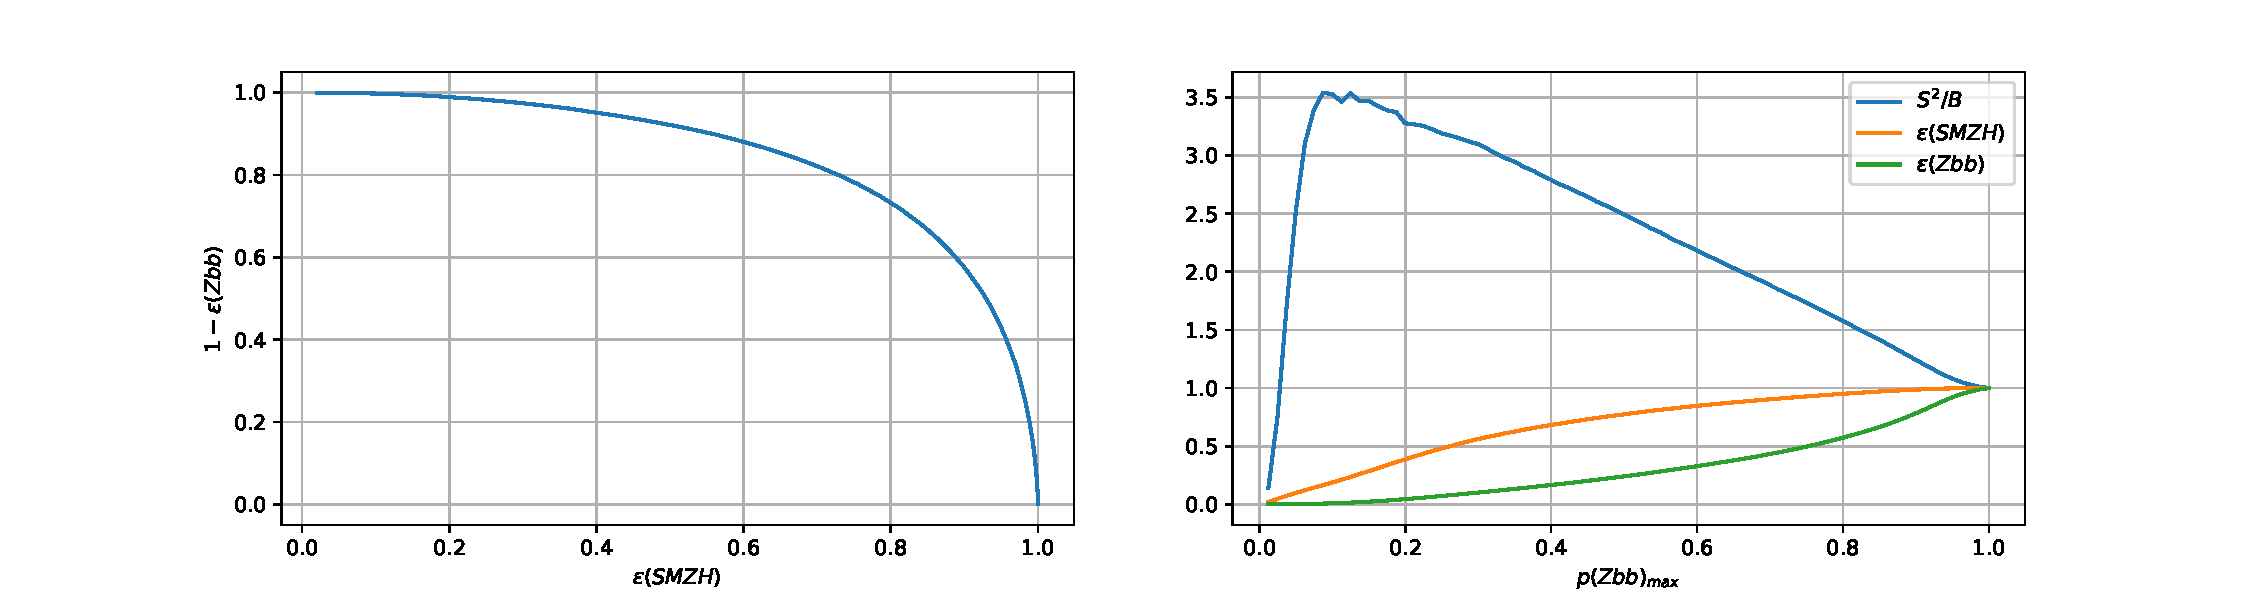
\includegraphics[width=0.8\textwidth]{plots/bkg_cut_opt.pdf}
\caption{
\label{fig:s2_over_b}
Optimisation analysis to determine the maximum value of $p(Z b\bar{b})$ for events
considered in the analysis. (left) {\it ROC} curve for $Z b\bar{b}$ vs SM $Z H$
separation. (right) Regularised $\varepsilon^2(SM Z H) /
\varepsilon(Zb\bar{b})$ as a function of the $p(Z b\bar{b})_{max}$.
}
\end{figure}

For this exploratory study, we only considered four BSM benchmarks, varying $c_{\sss HW}$ and testing the
sensitivity to each of these benchmarks using a dedicated set of kinematic
discriminants. While the design of an optimal discriminant that continuously depends on
the BSM parameters is beyond the scope of this work, we investigated the degree of
correlation between the BSM discriminants for each of the scenarios.
Figure~\ref{fig:bdt_corr} shows the linear correlation coefficient between $p(BSM)$ for
each of the four scenarios, evaluated on SM $Z H$ production events. The $p(BSM)$
BDT outputs estimate the likelihood for an event to come from each of the considered BSM
scenarios.
As it can be seen,
the linear correlation varies between 0.3 and 0.96, and it increases as the distance
between the benchmark points decreases. This suggests that the information used to
discriminate the different benchmarks is similar, but that optimal results are obtained
when a specific benchmark is targeted.

%% \red{everything below, inlcuding table, overlaps with the stats analysis sections -- need
%%   to decide where to put it} 
%% Finally, we compare the selection efficiency of selecting events according to the $p(Z
%% b\bar{b})$ discriminant trained to separate $Z b\bar{b}$ production from the SM $Z H$
%% production. \red{QUESTION: What are the BDT cuts used?} A difference in these figures
%% would directly affect any analysis based on STXS that are extrapolated to a larger phase
%% space assuming SM $Z 
%% H$ kinematics. As can be seen in Table~\ref{tab:bdt_efficiency}, relative differences in
%% efficiencies of the order of 20-50\% are observed. \red{In general, the sensitivity to any
%%   non-SM contribution to a measured cross section can only come from the events recorded
%%   in the fiducial volume, prior to any model-dependent extrapolations.} 
%
% \blindtext

\begin{figure}[h!]
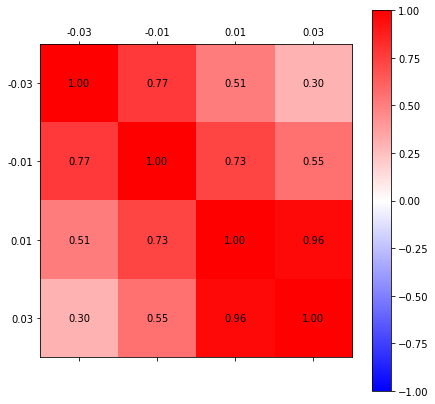
\includegraphics[width=0.35\linewidth]{plots/bdt_corr.png}
\caption{\label{fig:bdt_corr}A figure
  Linear correlation coefficient between $p(BSM)$ for
  each of the four scenarios, evaluated on SM $Z H$ production events.
  Row and columns are labelled by the value of $c_{\sss HW}$.
}
\end{figure}

%%% \newfloatcommand{capbtabbox}{table}[][\FBwidth]
%%% \begin{figure}[h!]
%%% \begin{floatrow}
%%% \ffigbox{%
%%% 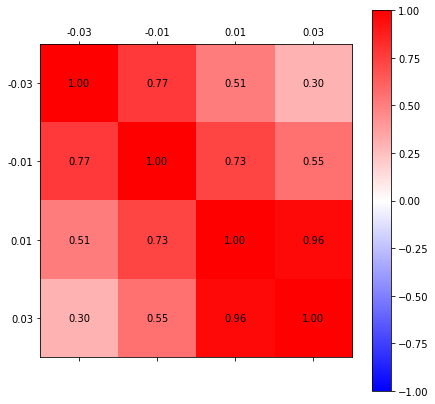
\includegraphics[width=0.8\linewidth]{plots/bdt_corr.png}
%%% }{%
%%%   \caption{\label{fig:bdt_corr}A figure
%%%   Linear correlation coefficient between $p(BSM)$ for
%%%   each of the four scenarios, evaluated on SM $Z H$ production events.
%%%   Row and columns are labelled by the value of $c_{\sss HW}$.
%%%   }%
%%% }
%%% \hspace{1cm}
%%% \capbtabbox{%
%%% \hspace{1cm}
%%% \begin{tabular}{||c|c||}
%%% sample & $\varepsilon$  \\
%%% \hline
%%% $c_{\sss HW} = 0.03$ & 0.14 \\
%%% $c_{\sss HW} = 0.01$ & 0.16 \\
%%% SM & 0.19 \\
%%% $c_{\sss HW} = -0.01$ & 0.23 \\
%%% $c_{\sss HW} = -0.03$ & 0.32 \\
%%% \end{tabular}
%%% \hspace{1cm}
%%% \vspace{1.2cm}
%%% }{%
%%%   \caption{
%%%   \label{tab:bdt_efficiency}
%%%   Selection efficiency for the $p(Z b\bar{b})$ selection for different scenarios. The
%%%   efficiency is computed for events in the fiducial volume defined in Table~\ref{tab:FiducialXS}.
%%%   \red{can we add the efficiency for Zbb to show how well it rejects and also use the number later in the text?}
%%%   }%
%%% }
%%% \end{floatrow}
%%% \end{figure}

% \end{document}
% \begin{figure}[h!]
% \centering
% 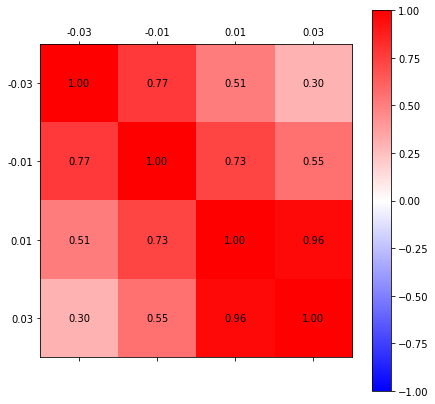
\includegraphics[width=\linewidth]{plots/bdt_corr.png}
% \caption{
% \label{fig:bdt_corr}
% Linear correlation coefficient between $p(BSM)$ for
% each of the four scenarios, evaluated on SM $Z H$ production events.
% Row and columns are labelled by the value of $c_{\sss HW}$.
% }
% \end{figure}
%
% \begin{table}
% \centering
% \begin{tabular}{||c|c||}
% sample & $\varepsilon$  \\
% \hline
% $c_{\sss HW} = 0.03$ & 0.14 \\
% $c_{\sss HW} = 0.01$ & 0.16 \\
% SM & 0.19 \\
% $c_{\sss HW} = -0.01$ & 0.23 \\
% $c_{\sss HW} = -0.03$ & 0.32 \\
% \end{tabular}
% \caption{
% \label{tab:bdt_efficiency}
% Selection efficiency for the $p(Z b\bar{b})$ selection for different scenarios. The
% efficiency is computed for events in the fiducial volume defined in Table~\ref{tab:FiducialXS}.
% }
% \end{table}
%
%

%%% Local Variables:
%%% mode: latex
%%% TeX-master: "STXSvsSpecificEFTAna"
%%% End:

%  

\subsection{STXS binning}

The generated samples for all signal benchmarks ($C_{HW}=???$) as well as the backgrounds (SM $pp \to ZH, H\to b\bar{b}$ and $pp\to Zb\bar{b}$) are categorized according to the STXS proposal for the $VH$ channel in Ref.~\cite{deFlorian:2016spz}. Within this framework, different regions of the phase space --referred to as ``bins'' for simplicity-- are defined, with the purpose of optimizing the sensitivity of the measurements while at the same time minimizing their dependence on theory assumptions. The different STXS bins are defined specifically for each Higgs production mode. For the process of interest
for the present exercise ($pp \to ZH \to \ell^+ \ell^- b\bar{b}$) the different stages of the categorization and the resulting bins are summarized as follows (see \cite{deFlorian:2016spz} for details):
%
\begin{itemize}
{\item  {\bf Stage 0:} Events with $\left|y_H\right| <2.5$ are selected.}
%
{\item {\bf Stage 1:} $ZH$ production is splitted into production via $q\bar{q}$ or $gg$ initial states. Our process sample was generated at LO and only contains $q\bar{q}\to ZH$ events. Events are subsequently classified according to the value of $p_T^Z$ and number of extra jets\footnote{JETS ARE DEFINED AS?} in the event as follows:
%
\vspace{0.25cm}
%
\begin{center}
${\bf \underline{q\bar{q}\to ZH}}$
\end{center}
\begin{eqnarray}
p_T^Z \in& [0,150]~\mathrm{GeV},& \nonumber\\
%
p_T^Z \in& [150,250]~\mathrm{GeV}&(0\mbox{-}\mathrm{j}),\\
%
p_T^Z \in& [150,250]~\mathrm{GeV}&(\geq 1\mbox{-}\mathrm{j}),\nonumber\\
%
p_T^Z >&250~\mathrm{GeV}.\nonumber&
\end{eqnarray}
}
%
%
{\item {\bf Stage 2:} On this last stage the low $p_T^Z$ bins are further separated according to the number of extra jets, while the high-$p_T^Z$ region is split at 400 GeV. The final set of STXS bins that apply in our case are the following six:
%
\vspace{0.25cm}
%
\begin{center}
${\bf \underline{q\bar{q}\to ZH}}$
\end{center}
\begin{eqnarray}
p_T^Z \in& [0,150]~\mathrm{GeV}&(0\mbox{-}\mathrm{j}),\nonumber\\
%
p_T^Z \in& [0,150]~\mathrm{GeV}&(\geq 1\mbox{-}\mathrm{j}),\nonumber\nonumber\\
%
p_T^Z \in& [150,250]~\mathrm{GeV}&(0\mbox{-}\mathrm{j}),\\
%
p_T^Z \in& [150,250]~\mathrm{GeV}&(\geq 1\mbox{-}\mathrm{j}),\nonumber\\
%
p_T^Z \in& [250,400]~\mathrm{GeV},&\nonumber\\
%
p_T^Z >&400~\mathrm{GeV}.\nonumber&
\end{eqnarray}
}
\end{itemize}
%
{[\bf EXPLAIN THE USE OF THE BDT VARIABLE TO REJECT BACKGR AFTER THE BDT SECTION IS DONE]}
{[\bf Figs: $S^2/B$ for the different benchmarks. Define S as new physics only?} 




\section{Statistical Hypothesis testing}
\label{sec:test}
%All!
%!TEX root = /Users/Ken/Work/Projects/LesHouches2017/STXSvsEFT/repo/LHStxsVsEft/Documentation/STXSvsSpecificEFTAna.tex
A statistical analysis is carried out to estimate the sensitivity to SMEFT effects in Higgs boson interactions of the STXS measurements compared to that of a dedicated analysis using a multivariate classifier. To this effect, a simple significance analysis is used based on the {\sc RooStats} framework~\cite{Moneta:2010pm} which determines the expected signifiance using an asymptotic calculator with nominal Asimov data sets and a one-sided profile likelihood. 

Naturally, a few approximations have been made. No systematic uncertainties have been considered, even if the generated events have been smeared to reflect the limited resolution and corrected for the finite efficiencies of $b$-tagging. The measurement in the STXS bins requires an extrapolation from the measured phase space, which includes those selections applied specifically to reject backgrounds, in this case from the $Z b\bar{b}$ process. In case of the present analysis this is achieved using a BDT specifically trained to select $H\to b\bar{b}$ over $Z b\bar{b}$ events. For the STXS analysis, a BDT cut of $<$0.1 is applied, retaining 18.6\% of all SM Higgs events but less than 1\% of the $Z b\bar{b}$ background. For the BDT analysis targeting EFT operators, two settings are explored: Using the same BDT requirement as in the STXS analysis and additionally using a selection requirement of the BDT of $<$0.055 (and 0.06 for $c_{\sss HW} <0$) which leads to similar acceptances as in the STXS case. 

In a real-life analysis, the effects of using the BDT-selection would have to be accounted for. Herein, it is assumed, that these are perfectly known for both SM and BSM events with $c_{\sss HW} \neq 0$. Different acceptances of SM and BSM however can play a role, when testing for BSM physics in the STXS phase space, to which the events selected on detector level have been extrapolated assuming the SM acceptances alone. For information, the acceptances of the BDT-selection for both, SM and BSM events with $c_{\sss HW} \neq 0$ are summarized in Table~\ref{tab:bkg_acceptance}. Similar considerations apply to the dedicated SMEFT-BDT analysis: the acceptances of signal and backgrounds need to be modelled well and also the distribution of the BDT classifier distribution needs to be well understood. Both is assumed to be the case in the following.

The acceptance of the first BDT selection is summarized in Table~\ref{tab:bkg_acceptance}. The acceptance for the SM Higgs can (depending on the BDT cut) be indeed very similar for both STXS BDT and EFT optimized-BDT (around 18\%). The acceptance for events with a Wilson coefficent $c_{\sss HW}=0.03$ is larger than that by about a factor of 1.5 whilst it is smaller by the 25\% for $c_{\sss HW}=-0.03$. For the samples produced with a smaller Wilson coefficient, $c_{\sss HW} = \pm0.01$, the acceptances are slightly closer to the SM Higgs scenario, which is expected since for $c_{\sss HW} \varinjlim 0$ the SM is restored. The smaller the Wilson coefficients, the smaller issues from acceptance effects. 
\red{I would stress that such acceptance differences are normally present in the
  experimental analysis, and are not accounted for}

\begin{table}[!h]
\begin{center}
{\scriptsize
\begin{tabular}{|l|c|c|c|}
\hline  
Sample		&  STXS: Acceptance (BDT$_{\mathrm{SM}}$) [\%] &  BDT: Acceptance (BDT$_{\mathrm{SM}}$, &  BDT: Acceptance (BDT$_{\mathrm{SM}}$, 	\\ 
		&  &  same as STXS SM-acceptance) [\%] &  same cut as STXS-BDT) [\%] 	\\ \hline

Higgs (BDT for $c_{\sss HW} = +0.03$) & 	18.6	&  18.5	& 29.6	\\
Higgs (BDT for $c_{\sss HW} = -0.03$)& 	18.6	&  18.3	& 33.1	\\
Higgs (BDT for $c_{\sss HW} = +0.01$)& 	18.6	&  18.6	& 33.4	\\ 
Higgs (BDT for $c_{\sss HW} = -0.01$)& 	18.6	&  19.8	& 34.2	\\ \hline

$c_{\sss HW} = 0.03$ &	31.1 & 31.8& 42.7\\
$c_{\sss HW} = -0.03$ &	14.4 &13.4& 28.2\\

$c_{\sss HW} = 0.01$ &	22.9	&23.0& 37.9\\
$c_{\sss HW} = -0.01$ &	15.9	&17.2& 31.7\\ \hline

$Z b\bar{b}$ &	<1.0	& $\sim$1.0 & $\sim$3.0\\ \hline

\end{tabular}
}
\vskip0.5truecm
\caption{Acceptances (in \%) of the first BDT selection, meant to separate $H\to b\bar{b}$ from $Z b\bar{b}$ production.}
\label{tab:bkg_acceptance}
\end{center}
\end{table} 

After application of the BDT requirements to reject $Z b\bar{b}$, either the STXS binning is applied or the distribution of the BDT classifier to select events with $c_{\sss HW} \neq 0$ against $H\to b\bar{b}$ events is evaluated. Either the STXS binning or the BDT classifier is used to estimate the sensitivity to new physics as expressed by the Wilson coefficients. Three different luminosity scenarios are investigated: the full Run-2 results, corresponding to 150 fb$^{-1}$, the integrated luminosity projected for LHC Run-3 (300 fb$^{-1}$) and the expected data collected at the High-Luminosity LHC (3000 fb$^{-1}$). The significance is determined simultaneously in the 6 STXS bins (see Section~\ref{sec:stxs}) and in the BDT discriminant (10 bins with sizeable entries, with more bins not changing the significance and less bins reducing it slightly). For both, STXS and BDT discriminant, no uncertainties on the shapes of these distributions are assumed. Figure~\ref{fig:hypotest} depicts the distributions used as inputs in the SXTS (left) and the BDT (right) case for 300 fb$^{-1}$. The SM hypothesis ($Z b\bar{b}$ + $H\to b\bar{b}$) is shown as blue line, whereas the BSM signal with $c_{\sss HW} = 0.03$ is shown as red line. They are added in the signal+background hypothesis which is depicted as dashed black line. A simple significance test for the signal+background hypothesis is carried out using the {\sc RooStats} framework~\cite{Moneta:2010pm} for these binned distributions. 
 
 
\begin{figure}[htb]
\centering
      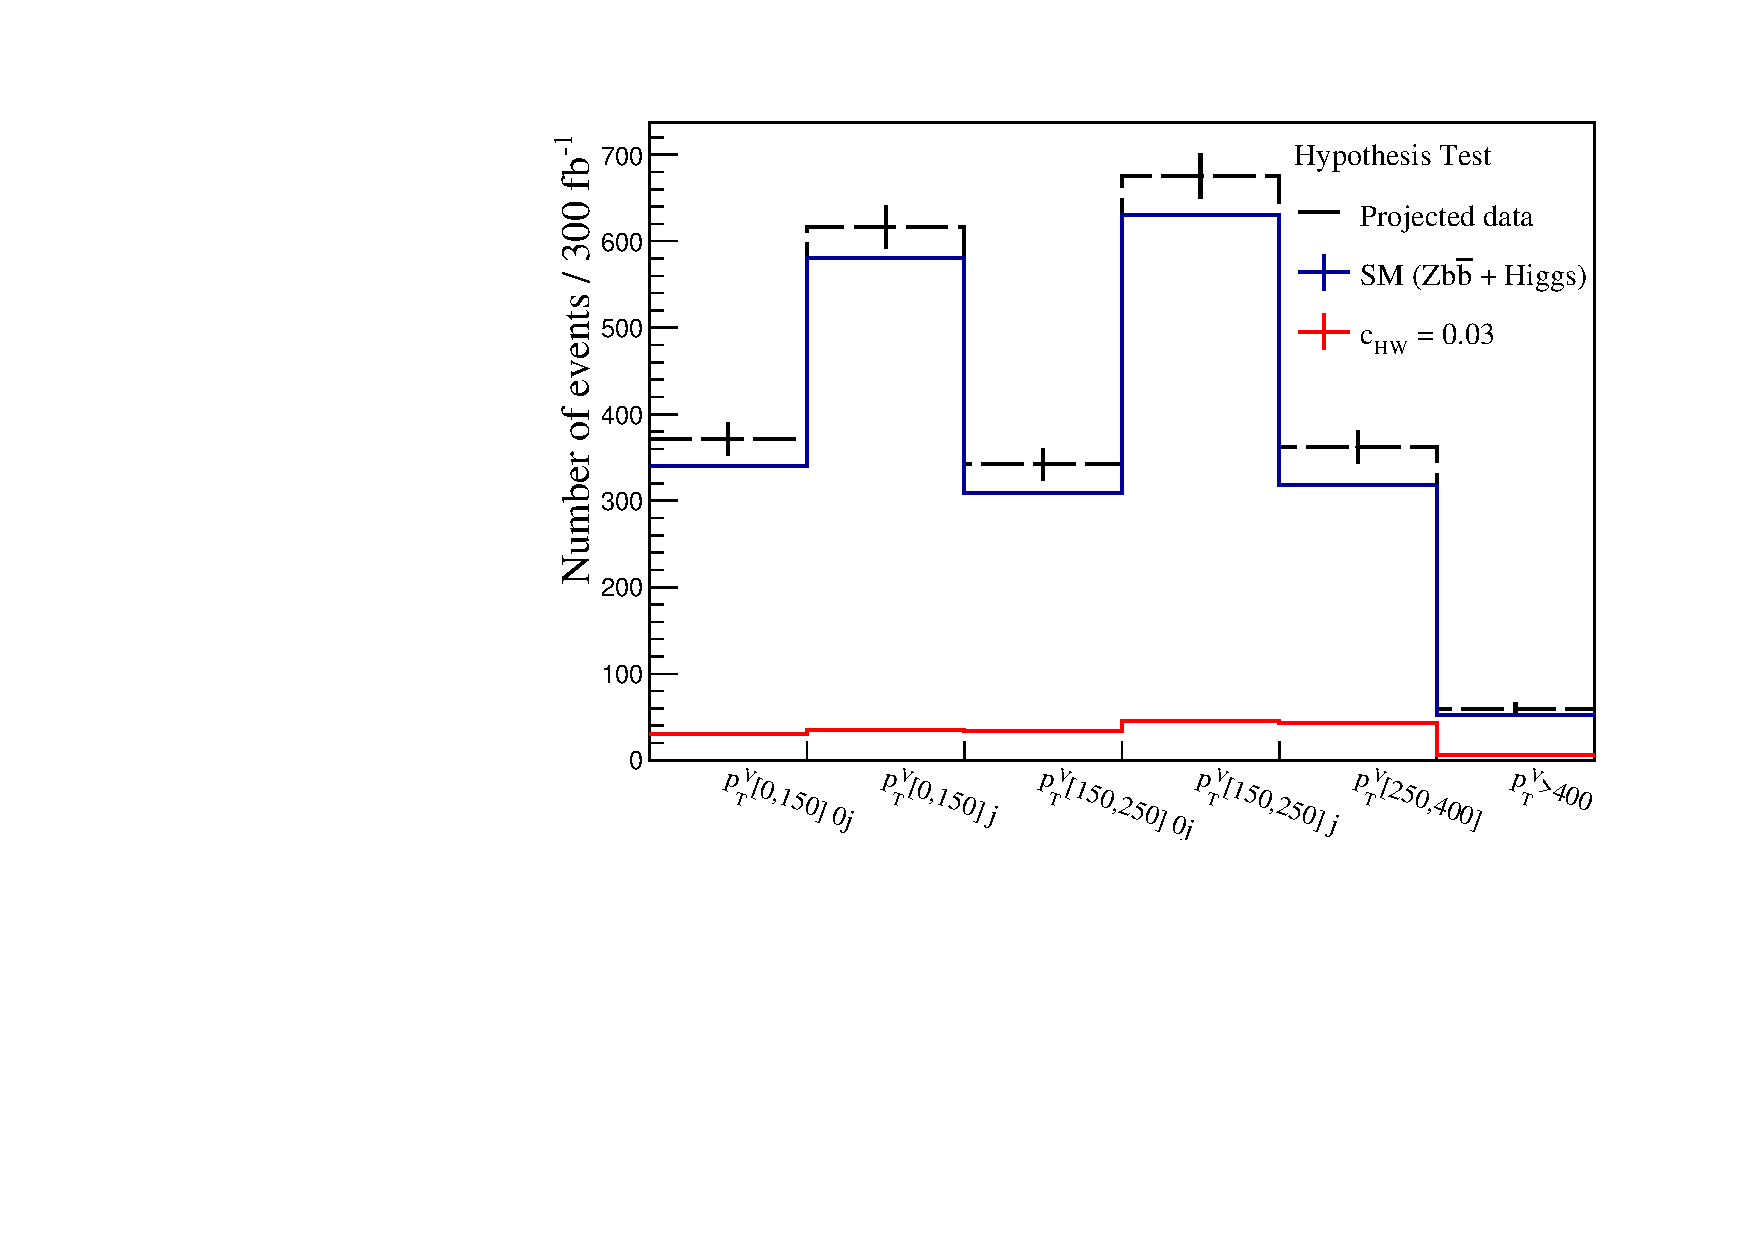
\includegraphics[width=0.45\textwidth]{plots/HypoTest_STXS.pdf}
      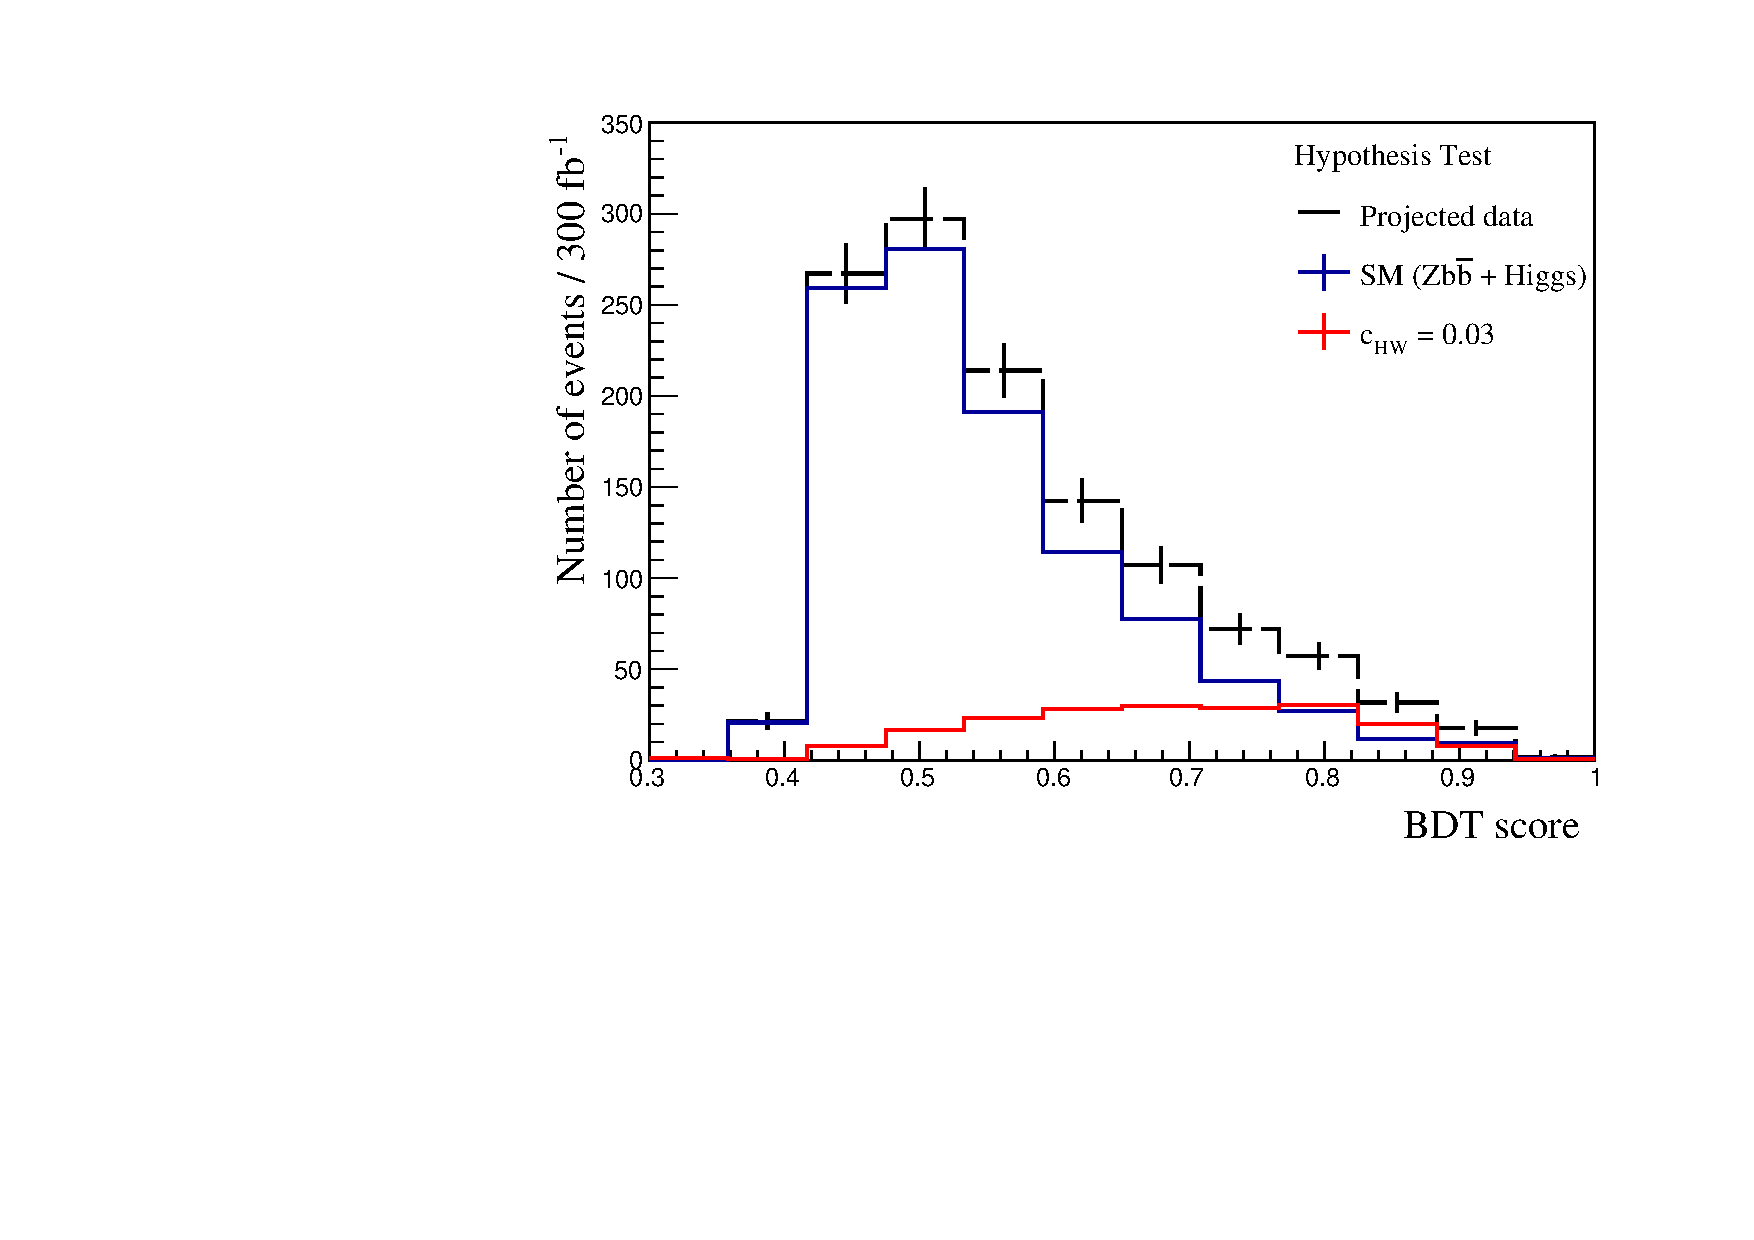
\includegraphics[width=0.45\textwidth]{plots/HypoTest_BDT.pdf}
      \caption{Predicted number of events selected for 300 fb$^{-1}$. Since the acceptance extrapolation into the STXS phase space does not change the available data statistics, it it not applied here, i.e. the distributions are shown after the first cut on the BDT classifier to reject the $Z b\bar{b}$ background.}
\label{fig:hypotest}
\end{figure}

To get a feeling of how realistic the scenario investigated herein is, the significance of a Higgs discovery in the STXS scenario is also investigated in addition to investigating the BSM sensitivity. The expected significances for the 2-lepton channel investigated here are 1.9 for ATLAS~\cite{Aaboud:2017xsd} and 1.8 for CMS~\cite{Sirunyan:2017elk} for $\sim$36 fb$^{-1}$. This is about what is expected from the simplified studies herein, which do not account for systematic uncertainties (which make up half the total uncertainty in the measurements) but are not optimized for a Higgs observation. The expected significance of a Higgs signal compared to a background (i.e. $Z b\bar{b}$) only sample is shown in Table~\ref{tab:significances}.

Table~\ref{tab:significances} also summarizes the significances found for the three luminosity scenarios for the hypothesis tests for the STXS and the BDT approach for Wilson coefficients of $c_{\sss HW} = \pm0.03$ and $c_{\sss HW} = \pm0.01$. In the case of the BDT approach and $c_{\sss HW} = \pm0.03$, three alternatives were tested. For these either the first BDT selection with the same STXS SM-acceptance or the same BDT cut as STXS are investigated and in addition a non-optimal BDT discriminant is used, that was trained not on the targeted Wilson coefficient but on it's opposite charge equivalent. 

%Surprisingly, the BDT approach that dedicatedly targets the BSM encapsulated by the Wilson coefficient does perform rather similarly to the STXS, independently of which $Z b\bar{b}$ rejection setting was used. As expected, the usage of the non-optimal BDT discriminant reduces the expected significance significantly. This can be understood from the fact that $ZH$ production at LO, being a $2\to2$ process, has only two kinematic degrees of freedom. Large kinematic effects from the EFT may be so striking in this case that the BDT is unable to provide significantly more separation power. However, for the smaller Wilson coefficient of $c_{\sss HW} = \pm0.01$, the BDT performs slightly better compared to the STXS, this difference seemingly increases as the deviation from SM predictions decreases as the greatest disparity in performance exists in the $c_{\sss HW} = -0.01$ benchmark, which differs the least from the SM. It appears that the BDT is better able to provide discrimination in the case where the new physics contribution is more evenly distributed across the phase space, as opposed to the extreme cases where the high $p_T$ region is dominated by new physics. This however would need to better studied.

 %c_{\sss HW} = \pm 0.03 \text{ and } \pm0.01\,,

\begin{table}[!h]
\begin{center}
{\scriptsize
\begin{tabular}{|l|c|c|c|c|c|c|c|c|c|}
\hline  
Hypothesis test		&  Full Run-2 (150 fb$^{-1}$) 	& LHC Run-3 (300 fb$^{-1}$) 	& HL-LHC  (3000 fb$^{-1}$) \\ \hline

STXS: Higgs discovery	& 		3.01 &  	3.70
			& 8.06 \\ \hline

STXS: $c_{\sss HW} = 0.03$ &		6.44 	&	8.82	& 26.46\\
STXS: $c_{\sss HW} = -0.03$ &		1.66&	2.24 &  257 7.19\\
%%------------------------------
BDT: $c_{\sss HW} = 0.03$ (STXS SM-acceptance)&		 6.29&	8.58 & 25.61\\
BDT: $c_{\sss HW} = -0.03$ (STXS SM-acceptance)&		1.80&	2.44& 7.24\\ \hline
%%------------------------------
BDT: $c_{\sss HW} = 0.03$ (same BDT cut as STXS)&	6.17&	8.64 & 27.03\\
BDT: $c_{\sss HW} = -0.03$ (same BDT cut as STXS)&	1.74 &	2.08 & 7.50\\ \hline
%%------------------------------
BDT: $c_{\sss HW} = 0.03$ (alt BDT cut)		&4.40	&	6.15	&19.18\\
BDT: $c_{\sss HW} = -0.03$ (alt BDT cut)	&1.44	&	2.41	& 6.69\\ \hline
%%------------------------------
STXS: $c_{\sss HW} = 0.01$ &		2.26		&	3.04			& 8.78\\
STXS: $c_{\sss HW} = -0.01$ &		1.08		&	1.46			& 4.30\\ 
%%------------------------------
BDT: $c_{\sss HW} = 0.01$ &		2.62		&	3.07			& 8.90\\
BDT: $c_{\sss HW} = -0.01$ &		1.44		&	1.99			& 6.10\\ \hline
\end{tabular}
}
\vskip0.5truecm
\caption{Expected significances for different scenarios.}
\label{tab:significances}
\end{center}
\end{table} 



\section{Conclusions}
\label{sec:conclusions}
%!TEX root = /Users/Ken/Work/Projects/LesHouches2017/STXSvsEFT/repo/LHStxsVsEft/Documentation/STXSvsSpecificEFTAna.tex
We have performed an exploratory study comparing the sensitivity to higher dimensional operators of the proposed STXS measurements in $ZH$ production to an optimised analysis exploiting multivariate methods. We considered four benchmark scenarios in which the $\mathcal{O}_{\sss HW}$ operator coefficient is set to values of $\pm 0.03$ and $\pm 0.01$. The former case corresponds to saturating existing limits from a global fit to LHC Run 1 data and precision electroweak measurements, while the latter case intends to showcase a scenario with smaller deviations from SM expectations. The sensitivity was quantified by the expected statistical significance against the SM hypothesis obtainable after a collected integrated luminosity of 150, 300 and 3000 fb$^{-1}$, taking into account the presence of the dominant SM background of $Zb\bar{b}$ production. The contribution of this background is efficiently mitigated by training a BDT classifier to distinguish this process from SM $ZH$ production and first cutting on this discriminant before performing the two alternative SM vs EFT significance analyses. The discriminant was able to effectively reduce this background contribution down by two orders of magnitude.

Overall, very large significances can be expected for the benchmarks saturating the current limits, while the benchmarks for the smaller Wilson coefficients are not likely to be identified beyond 3$\sigma$ until the High-Luminosity LHC run. We observe that the final performance of the BDT analysis does not differ significantly from the differential information in $Z$-boson $p_T$ offered by the STXS, with the exception of the $c_{\sss HW}=-0.01$ case, which predicts the smallest deviation from the SM case. Here, the discriminating power of the BDT output over the differential $p_T$ distributions becomes apparent, suggesting that once the sensitivity of the STXS measurements is saturated, moving towards optimised multivariate methods remains well-motivated. The exercise was performed in a simplified situation, largely ignoring detector effects besides a parametrised $b$-jet smearing implementation and $b$-tagging efficiency corrections as well as all other potential sources of systematic uncertainty. We leave a more thorough investigation, including these effects as well as the possibility of including other significant backgrounds to a follow-up study. 

By comparing the optimised BDT discriminants for the different EFT benchmarks, we conclude that there is significant information overlap between them but that some parameter dependence remains, meaning that one would benefit from a parametrised learning approach in which the new physics parameter is also fed in as an input to the discriminant training. This can be understood from the presence of both an interference and squared contribution of the EFT $ZH$ amplitude in the new physics signal. The shape of EFT squared contribution has the benefit of being independent of the value of the Wilson coefficient, while the relative impact of the interference term depends very much on this value. In the `large' $c_{\sss HW}$ benchmarks, the contribution from the quadratic term in the Wilson coefficient is clearly dominant at high energies, as evidenced by the positive relative contribution over the SM prediction for both $\pm0.03$ in the STXS overflow bin. On the other hand the $-0.01$ case consistently predicts a deficit with respect to the SM. The fact that the BDT outperforms for this benchmarks may imply that one can obtain better sensitivity using these methods for EFT signals in which the interference with the SM amplitude is significant, which may also be considered more `well-behaved' concerning the EFT expansion. However, this effect may also be caused by the greater loss in acceptance post $Zb\bar{b}$ BDT cut suffered by the negative $c_{\sss HW}$ benchmarks and should be further investigated.

One should bear in mind that in this first study, a rather kinematically simple process has been chosen in $ZH$ production, in which the $Z$-boson $p_T$ is very strongly correlated to the energy flow through the production vertex, in which the EFT effects occur. It is therefore not surprising that we do not observe a huge difference in significance in this case. Further investigations concerning a comparison between BDT and STXS for less well-defined kinematic environments would be also interesting, \emph{e.g.}, for other $2\to3$ production modes such as vector boson fusion or $t\bar{t}$ associated production.  Furthermore, it should be noted that although our BDT analysis is touted as an `optimised' discriminating method, the fully potential of the BDT information was not exploited in this analysis. In short, by cutting on the SM vs $Zb\bar{b}$ variable and fitting on the resulting one-dimensional discriminant, some amount of exclusion power was sacrificed for the sake of simplicity. In the ideal case, a two-dimensional fit on the initial BDT classifier would be performed, an exercise which we leave for the follow-up study.
\red{I would add a short discussion of the acceptance effects that are usually not accounted for.}




\section*{Acknowledgments}

We thank the organizers and conveners of the Les Houches workshop, ``Physics
at TeV Colliders'', for a stimulating meeting. This work has received funding from the European Union's Horizon 2020 research and innovation programme / ERC Grant Agreement n. 715871. K. M. is supported in part by the Belgian Federal Science Policy Office through the Interuniversity Attraction Pole P7/37 and by the European Union’s Horizon 2020 research and innovation programme under the Marie Sk\l{}odowska-Curie grant agreement No. 707983.


%\vfil\eject


\bibliography{STXSvsSpecificEFTAna}
\bibliographystyle{utcaps}
%\bibliographystyle{lesHouches}
\end{document}
